\chapter{Аналитический раздел}

\section{Допустимые положения пальцев рук}
\hspace{0.6cm}Каждый палец, кроме первого, состоит из проксимальной (более приближенной к лучезапястному суставу), медиальной (средней) и дистальной (наиболее удалённой от лучезапястного сустава) фаланг, а большой палец - из проксимальной и дистальной фаланги. Пальцы нумеруются с единицы, начиная с большого пальца.  

\begin{figure}[ht!]
	\centering
	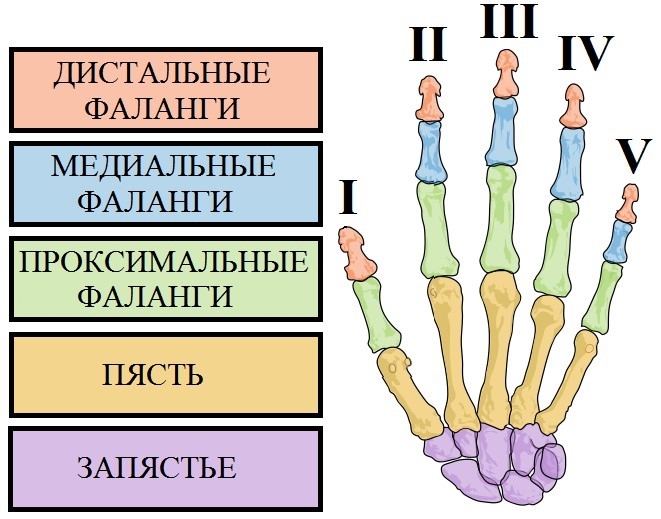
\includegraphics[scale=0.4]{hand_bones.jpg}
	\caption{Составные части кисти}
	\label{fig:hand_bones}
\end{figure}

\hspace{0.6cm}В каждом из суставов пальцев кисти выполняется сгибание и разгибание, но только в пястных суставах - отведение и приведение. Движения могут быть следующими: активными (вызванными собственными сокращениями мышц кисти) и пассивными (вызванными внешней причиной). Большой палец, который имеет наиболее сложную структуру, способен на такие движения, как сгибания и разгибание, отведение и приведение, а также противопоставление при помощи пястной кости. В пястно-фаланговом и межфаланговом суставах большого пальца возможны только сгибание и разгибание.

\hspace{0.6cm}Простые движения кисти приведены на рисунках \ref{fig:hand_motions} и \ref{fig:hand_extension}. Амплитуда сгибания/разгибания и отведения/приведения измеряется из нейтрального положения, при котором ось кисти, проходящая через средний палец и третью пястную кость, коллинеарна продольной оси предплечья.  

\begin{figure}[ht!]
	\centering
	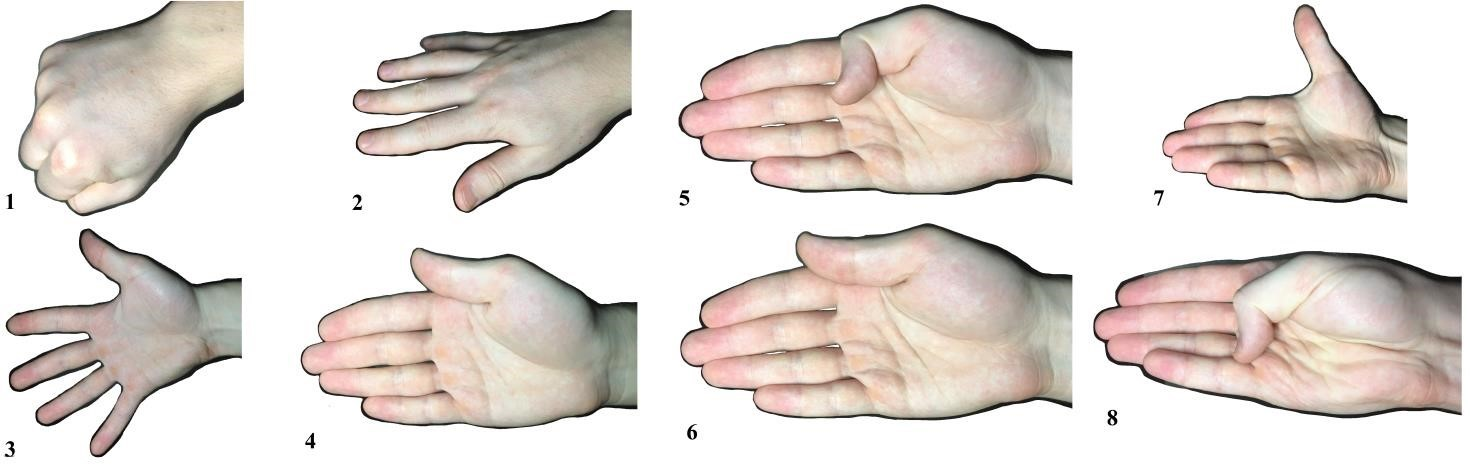
\includegraphics[scale=0.65]{hand_motion.jpg}
	\caption{Движения кисти. 1. Сгибание пальцев. 2. Разгибание пальцев 3. Отведение пальцев. 4. Приведение пальцев. 5. Сгибание большого пальца 6. Разгибание большого пальца. 7. Отведение большого пальца. 8. Противопоставление большого пальца}
	\label{fig:hand_motions}
\end{figure}

\begin{figure}[ht!]
	\centering
	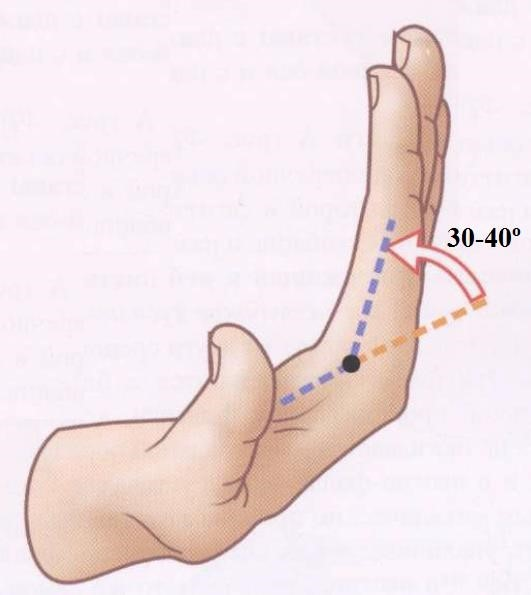
\includegraphics[scale=0.4]{hand_extension.jpg}
	\caption{Активное разгибание в пястно-фаланговом суставе}
	\label{fig:hand_extension}
\end{figure}

\hspace{0.6cm}Вокруг вертикальной оси в горизонтальной плоскости осуществляются вращение внутрь (пронация) и наружу (супинация) большого пальца вместе с пястной костью при помощи пястно-запястного сустава. Большой палец при сгибании вокруг сагиттальной оси во фронтальной плоскости смещается в сторону ладони, при этом возможно противопоставление остальным пальцам. Движение вокруг фронтальной оси определяется как приведение и отведение большого пальца.

\newpage

Простые движения состоят из:
\begin{itemize}
	\item «Сгибания в лучезапястном суставе» или «Разгибания в лучезапястном суставе»; 
	\item «Отведения в лучезапястном суставе» или «Приведения в луче-
запястном суставе»;  
	\item «Сгибания пальцев» или «Разгибания пальцев»  (большой палец 
рассматривается отдельно); 
	\item «Отведения пальцев» или «Приведения пальцев» (большой палец рассматривается отдельно); 
	\item «Сгибания большого пальца» или «Разгибания большого пальца»; 
	\item «Отведения большого пальца» или «Приведения большого пальца»; 
	\item «Противопоставления большого пальца». 
\end{itemize}

\hspace{0.6cm}Были составлены таблицы \ref{tab:amplitude_palm} и \ref{tab:amplitude_finger} амплитудных углов кисти и пальцев от нейтрального положения. Также, принимая во внимание факт, что движения отведения или приведения совершаются самостоятельно только проксимальными фалангами, все другие фаланги данного движения самостоятельно не выполняют и являются ведомыми. II палец отличается способностью производить отведение в 60º от начального положения, сохраняя возможность выполнять приведение и отведение в диапазоне 30º.

\begin{table}[ht!]
	\caption{Угловая амплитуда движений ладони}
	\label{tab:amplitude_palm}
	\begin{center}
		\begin{tabular}{|c|c|}
			\hline
			\bf{Движение} & \bf{Амплитуда, º}\\\hline
			Сгибание & 80 - 85\\\hline
			Разгибание & 70 - 85\\\hline
			Отведение & 15 - 25\\\hline
			Приведение & 30 - 45\\\hline
		\end{tabular}
	\end{center}
\end{table}

\begin{table}[ht!]
	\caption{Угловая амплитуда движений пальцев }
	\label{tab:amplitude_finger}
	\begin{center}
		\begin{tabular}{|c|c|c|c|c|c|c|}
			\hline
			\multicolumn{3}{|c|}{Движение} & Сгибание & Разгибание & Отведение & Приведение\\\cline{1-7}
			\multirow{7}*{Амп., º} & \multirow{3}*{\parbox[c]{1cm}{БП}} &  \parbox[c]{3cm}{Пястная кость и запястье} & 20 & !20 & 20 & 20\\\cline{3-7}
			& & \parbox[c]{3cm}{Проксимальная фаланга и пястная кость} & 50 & !50 & - & - \\\cline{3-7}
			& & \parbox[c]{3cm}{Дистальная и проксимальная фаланги} & 80 & !80+(20) & - & -\\\cline{2-7}
			& \parbox[c]{1cm}{II палец} & \parbox[c]{3cm}{Проксимальная фаланга и пястная кость} & - & - & 60 & !60\\\cline{2-7}
			& \multirow{3}*{\parbox[c]{1cm}{II, III, IV, V пальцы}} & \parbox[c]{3cm}{Проксимальная фаланга и пястная кость} & 90 & !90+(30) & 30 & 30\\\cline{3-7}
			& & \parbox[c]{3cm}{Медиальная и проксимальная фаланги} & 100 & !100 & - & -\\\cline{3-7}
			& & \parbox[c]{3cm}{Дистальная и медиальная фаланги} & 80 & !80 & - & -\\\cline{2-7}
			& \parbox[c]{1cm}{Ладонь} & \parbox[c]{3cm}{Ладонь и предплечье} & \multicolumn{2}{c|}{70} & \multicolumn{2}{c|}{80}\\\hline
		\end{tabular}
	\end{center}
\end{table}

\newpage

\section{Prolog}
\hspace{0.6cm}Prolog — язык и система логического программирования, основанные на языке предикатов математической логики дизъюнктов Хорна, представляющей собой подмножество логики предикатов первого порядка.
\hspace{0.6cm}Язык сосредоточен вокруг небольшого набора основных механизмов, включая сопоставление с образцом, древовидного представления структур данных и автоматического перебора с возвратами. Хорошо подходит для решения задач, где рассматриваются объекты (в частности структурированные объекты) и отношения между ними. Пролог, благодаря своим особенностям, используется в области искусственного интеллекта, компьютерной лингвистики и нечислового программирования в целом. В некоторых случаях реализация символьных вычислений на других стандартных языках вызывает необходимость создавать большое количество кода, сложного в понимании, в то время как реализация тех же алгоритмов на языке Пролог даёт простую программу, легко помещающуюся на одной странице.

\hspace{0.6cm}Prolog является декларативным языком программирования: логика программы выражается в терминах отношений, представленных в виде фактов и правил. Для того чтобы инициировать вычисления, выполняется специальный запрос к базе знаний, на которые система логического программирования генерирует ответы «истина» и «ложь». Для обобщённых запросов с переменными в качестве аргументов созданная система Пролог выводит конкретные данные в подтверждение истинности обобщённых сведений и правил вывода.
Иначе говоря, предикат можно определить как функцию, отображающую множество произвольной природы в множество булевых значений {ложно, истинно}. Задача пролог-программы заключается в том, чтобы доказать, является ли заданное целевое утверждение следствием из имеющихся фактов и правил.

\hspace{0.6cm}Основными понятиями в языке Пролог являются факты, правила логического вывода и запросы, позволяющие описывать базы знаний, процедуры логического вывода и принятия решений. В логическом программировании, как оно реализовано в прологе, используется только одно правило вывода — резолюция.
В языке пролог исходное множество формул, для которого ищется пустая резольвента, представляется в виде так называемых «дизъюнктов Хорна»:

\hspace{0.6cm}Программа на Прологе описывает отношения, определяемые с помощью предложений. Как и в любом другом языке, ориентированном на символьные вычисления, предложения выстраиваются из термов, которые в свою очередь подразделяются на атомы, числа, переменные и структуры.
\hspace{0.6cm}Структуры представляют собой совокупности термов, заключённые в круглые скобки, в том числе и другие структуры. Структура обозначается именем (функтором), которое располагается перед круглыми скобками.

book( 'Название', '2009', 'Спб', authors( 'Первый автор', 'Второй автор' ) ).

Ещё одной конструкцией являются списки, элементы которых заключаются в квадратные скобки. В основе списков в Пролог лежат связные списки.

\hspace{0.6cm}Правила в Прологе записываются в форме правил логического вывода с логическими заключениями и списком логических условий. В чистом Прологе предложения ограничиваются дизъюнктами Хорна.
\hspace{0.6cm}Факты в языке Пролог описываются логическими предикатами с конкретными значениями. Факты в базах знаний на языке Пролог представляют конкретные сведения (знания). Обобщённые сведения и знания в языке Пролог задаются правилами логического вывода (определениями) и наборами таких правил вывода (определений) над конкретными фактами и обобщёнными сведениями. Предложения с пустым телом называются фактами.


	
